%************************************************
\chapter{Stabilization by spatial variation of the drive}\label{ch:metronome-spin}

In this chapter, we consider a clean, i.e. disorder-free, Ising spin chain with periodic driving and explore the influence of a spatially inhomogeneous drive on the dynamics. Remarkably, we find the time dynamics to be very sensitive to even small variations of said drive. In fact, limiting the spatial inhomogeneity of the drive to a single site, while all other sites experience the same driving, is already sufficient to manipulate the lifetime of the time crystalline signatures greatly. For initial states polarized in $z$-direction, this remarkable sensitivity to even minor deviations of the driving field is closely related to the spontaneous symmetry breaking of the groundstate of the Ising model.
For generic states at high temperatures, the long-lived, period-doubled, oscillations are retained on the outer most spins only. We uncover the topological origin of this observation and exemplify it by slightly altering the systems geometry in way which removes the stabilization. 
These results persist in the presence of disorder or the addition of integrability breaking interactions. In summary, this work showcases a dramatic consequence of the long-range spatiotemporal order that is required to create a time crystal.

\newpage
\pdfbookmark[2]{Publication}{metronomespin-paper}
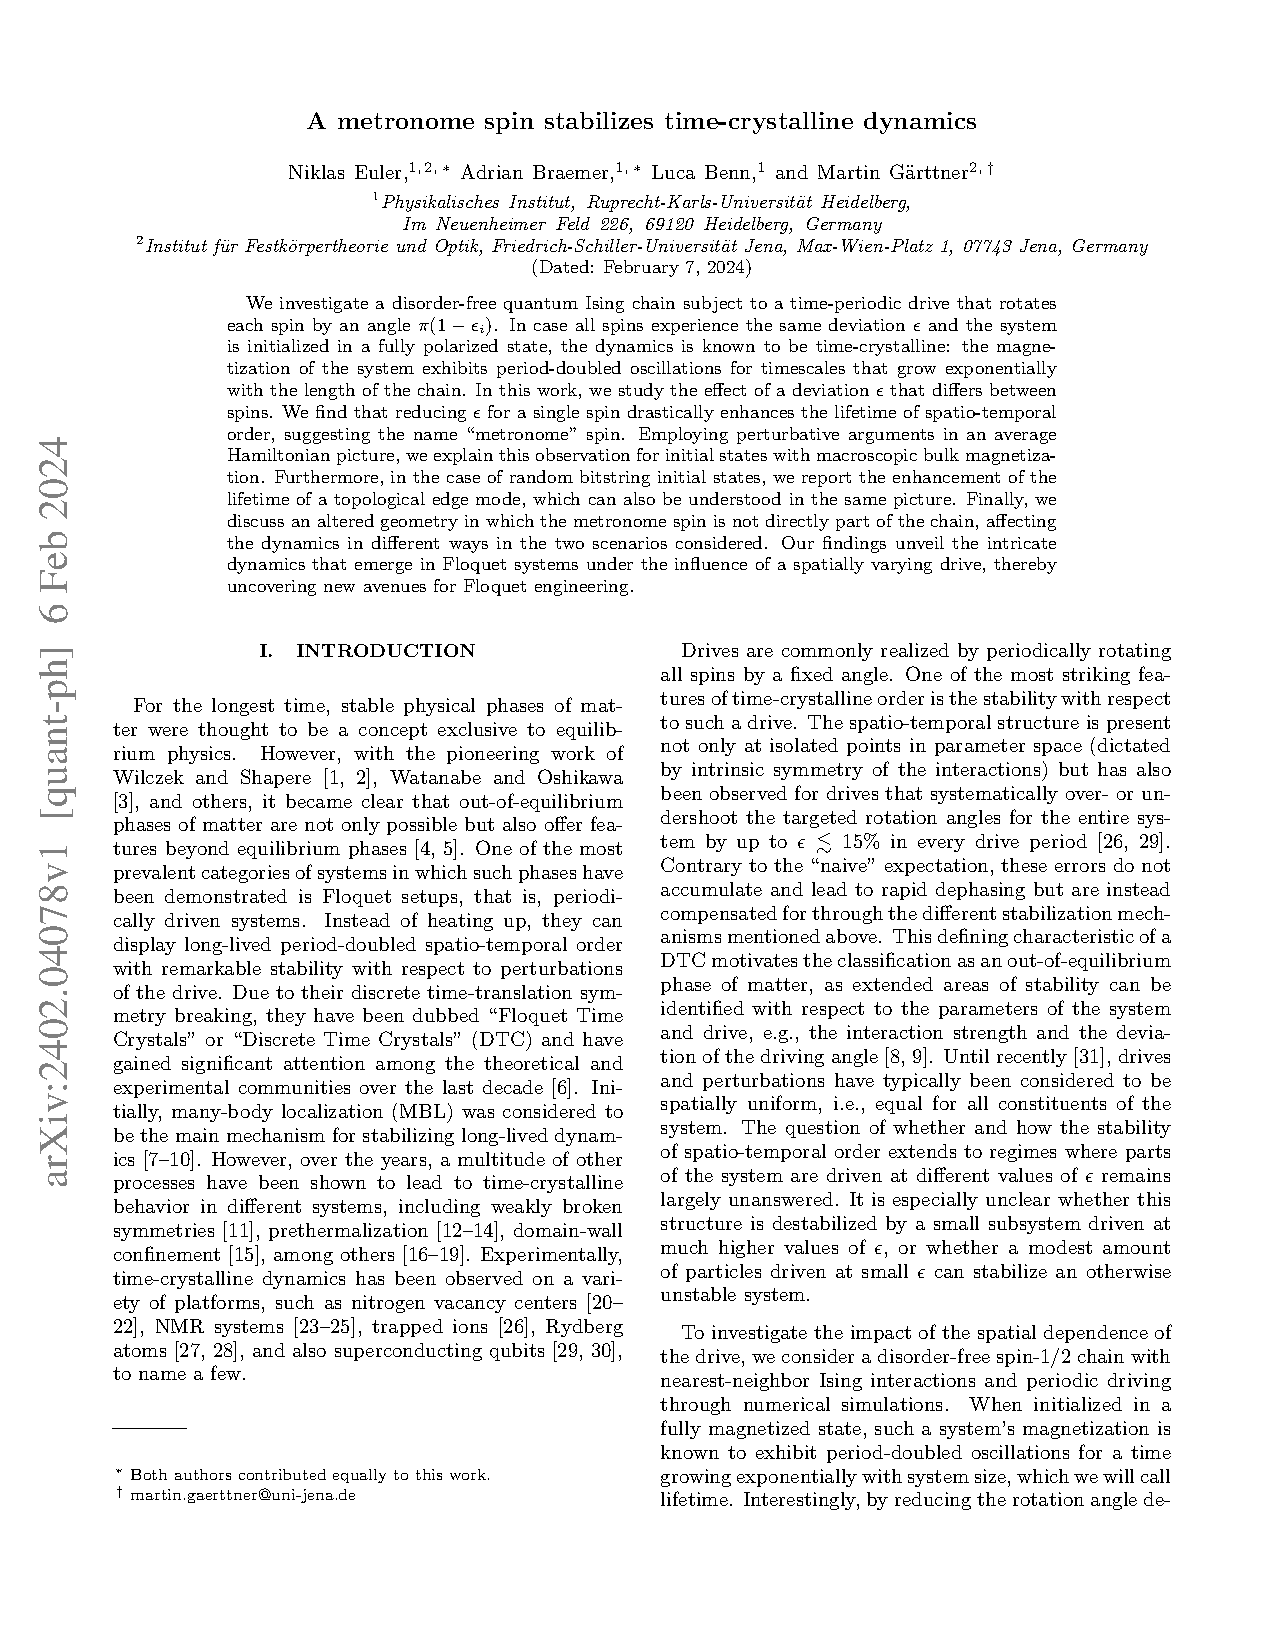
\includepdf[pages=-]{pub-Euler2024-MetronomeSpin}